\documentclass[12pt,a4paper]{report}

\usepackage{titlesec}
\usepackage{hyperref}

% Custom centered chapter format for front matter
\newcommand{\chaptercenter}[1]{%
  \titleformat{\chapter}[display]
    {\normalfont\bfseries\centering\fontsize{24}{28}\selectfont}
    {}
    {0pt}
    {} % No label
  \chapter*{#1} % Print chapter title
  \titleformat{\chapter}[display] % Restore main format
    {\normalfont\huge\bfseries}
    {\chaptertitlename\ \thechapter}
    {-1pt}
    {\huge}
  \titlespacing*{\chapter}{0pt}{15pt}{20pt} % Restore spacing
}

\usepackage{setspace}
\usepackage{geometry}
\usepackage{graphicx}
\usepackage{tocloft}
\usepackage{newtxtext} % Times New Roman
\usepackage{fancyhdr}
\usepackage{array}
\usepackage{longtable}
\usepackage[utf8]{inputenc}
\usepackage{booktabs}
\usepackage{amsmath}
\usepackage{enumitem}
\usepackage{hyperref}
\usepackage[numbers]{natbib}
\usepackage{placeins}
\usepackage{newtxmath}
\usepackage{adjustbox}
\usepackage{subcaption}
\usepackage[font=footnotesize,labelfont=bf,justification=centering]{caption}
\setcounter{secnumdepth}{3}
\setcounter{tocdepth}{3}

\geometry{margin=1in}
\setstretch{1.5}

% Page style setup
\pagestyle{plain} % Default to plain style (no header line) for front matter
\fancyhf{}
\renewcommand{\headrulewidth}{0.4pt} % Horizontal line in header
\cfoot{\thepage} % Page number in center footer for all pages

% Define fancy style for main content
\fancyhead[R]{\leftmark} % Chapter name in header (right)
\fancyfoot[C]{\textit{Department of Artificial Intelligence (AI) \& Data Science }} % Center footer
\fancyfoot[R]{\textit{\thepage}} % Right-aligned italic page number
\renewcommand{\chaptermark}[1]{\markboth{#1}{}} % Store chapter name for header
\renewcommand{\sectionmark}[1]{} % Ignore section name for header

% Switch to fancy style only for numbered chapters
\let\oldchapter\chapter
\renewcommand{\chapter}{\ifnum\value{chapter}>0 \clearpage\pagestyle{fancy}\fi\oldchapter}

% Roman page numbering for front matter
\pagenumbering{roman}

% Define title formats for front matter (centered for unnumbered chapters)
\titleformat{\chapter}[display]
{\normalfont\bfseries\centering\fontsize{24}{28}\selectfont}
{}
{0pt}
{}

\titleformat{\section}
{\normalfont\bfseries\fontsize{24}{28}\selectfont}
{}
{0pt}
{}

% For left aligned sections like Abstract, Contents etc.
\newcommand{\sectionleft}[1]{%
    \vspace*{1cm}%
    {\raggedright\bfseries\fontsize{24}{28}\selectfont #1\par}
    \vspace{1cm}
}

% Redefine title formats for main content
\titleformat{\section}
  {\normalfont\Large\bfseries} % Bold section headings
  {\thesection}{1em}{}
\titleformat{\subsection}
  {\normalfont\large\bfseries} % Bold subsection headings
  {\thesubsection}{1em}{}

\titleformat{\chapter}[display]
  {\normalfont\huge\bfseries}
  {\chaptertitlename\ \thechapter}
  {-1pt}
  {\huge}
\titlespacing*{\chapter}{0pt}{15pt}{20pt} % Reduced space above chapter title

\graphicspath{{images/}}

\begin{document}

%-------------------- Title Page ---------------------
\begin{titlepage}

    \centering
    \vspace{1cm}
    {\Huge \bfseries On-Device Conversational AI with a Post-Trained Qwen3.5 Model on Android \par}
    \vspace{0.5cm}
    {\Large  Submitted in partial fulfillment of the requirements of the degree\par}
    {\Large \bfseries BACHELOR OF ENGINEERING \par}
    {\large  IN\par}
     {\Large \bfseries \textbf{ARTIFICIAL INTELLIGENCE (AI) \& DATA SCIENCE}
 \par}
    \vspace{0.8cm}

    \textbf{By}
    \vspace{0.5cm}
 \begin{spacing}{1.2}
    {\large
    Rohit Swami \quad Roll No 1\\[6pt]
    Namish Sharma  \quad Roll No 2\\[6pt]
    Akhilesh Pottekat  \quad Roll No 3
    }
\end{spacing}
\vspace{0.25cm}
    \vfill
    {\large Supervisor\\[6pt]
    \textbf{Prof. / DR. guide name }}

    \vspace{0.5cm}
        
\includegraphics[width=0.45\textwidth]{sieslogo.png}\\[1em]

\begin{spacing}{1.8}
    {\fontsize{18pt}{18pt} \textbf{Department of Artificial Intelligence (AI) \& Data Science} \\ \fontsize{20pt}{20pt} \textbf{SIES Graduate School of Technology (Autonomous)} \\ Affiliated to University of Mumbai\\\textbf{Nerul, Navi Mumbai -- 400706 }\\
    \textbf{A.Y. 2026--27}}
    \end{spacing}
\end{titlepage}

\newpage

%-------------------- Certificate ---------------------
\chaptercenter{\Huge \textbf{CERTIFICATE} }
\vspace{1cm}
\begin{spacing}{1.8}
\thispagestyle{plain}
This is to certify that the project entitled \textbf{``On-Device Conversational AI with a Post-Trained Qwen3.5 Model on Android''} is a bonafide work of the following students, submitted to the SIES Graduate School of Technology in partial fulfillment of the requirement for the award of the degree of \textbf{Bachelor of Engineering} in \textbf{``Artificial Intelligence (AI) \& Data Science''}.
\end{spacing}
\vspace{0.5cm}

\begin{center}
\begin{tabular}{lll}
    Rohit Swami \hfill & Roll No 1 \\
    Namish Sharma \hfill & Roll No 2 \\
    Akhilesh Pottekat \hfill & Roll No 3 \\
\end{tabular}
\end{center}
\vspace{1.5cm}
\begin{center}
\begin{tabular}{>{\centering\arraybackslash}p{5cm} >{\centering\arraybackslash}p{5cm} >{\centering\arraybackslash}p{5cm} >
{\centering\arraybackslash}p{5cm} >{\centering\arraybackslash}p{5cm}}
    Dr. Arathi Boyannapalli& &  Dr. Neethu Anna Sabu \\
    \textbf{Supervisior}& & \textbf{Mini Project Coordinator} \\
    \vspace{2.2cm}
    Dr. Arathi Boyannapalli & & \vspace{2.2cm} Dr. K. Lakshmisudha \\
    \textbf{\textbf{Head of Department}} & & \textbf{Principal} \\
\end{tabular}
\end{center}

%-------------------- Approval ---------------------
\chaptercenter{\textbf{PROJECT REPORT APPROVAL}}
\thispagestyle{plain}
\vspace{1cm}

This Mini Project entitled `` \textbf{On-Device Conversational AI with a Post-Trained Qwen3.5 Model on Android} '' by following students is approved for the degree of \textbf{Bachelor of Engineering }in \textbf{Artificial Intelligence (AI) and Data Science}. \\
\begin{center}
\begin{tabular}{lll}
    \textbf{Rohit Swami} \hfill & \textbf{Roll No 1} \\
    \textbf{Namish Sharma} \hfill & \textbf{Roll No 2} \\
    \textbf{Akhilesh Pottekat} \hfill & \textbf{Roll No 3} \\
\end{tabular}
\end{center}

\begin{center}
  \vspace{1cm}  \textbf{Examiners}
\end{center}

\vspace{1.3cm}

\begin{flushright}
\begin{minipage}{0.5\textwidth}

1.\dotfill

\vspace{0.2cm}
\centering
(Internal Examiner Name \& Sign)

\vspace{1.62cm}

\raggedleft
2.\dotfill

\vspace{0.2cm}
\centering
(External Examiner Name \& Sign)

\end{minipage}
\end{flushright}

\vspace{1.5cm}

\begin{flushleft}
Date:

\vspace{0.8cm}

Place: SIES GST, Nerul, Navi Mumbai.
\end{flushleft}



\newpage

%-------------------- Acknowledgement ---------------------
\chaptercenter{\textbf{ACKNOWLEDGEMENT}}
\addcontentsline{toc}{chapter}{ACKNOWLEDGEMENT}
\thispagestyle{plain}
\vspace{1cm}

We would like to express our thanks to the people who have helped us the most throughout our project. We are grateful to our guide ( \textbf{Dr. Arathi Boyannapalli}) and coordinator, \textbf{Prof. Akshay A Jadhav }for nonstop support for the project. \vspace{0.4cm}
\\ A special thanks goes to each other who worked together as a team in completing the project, where we all exchanged our own interesting ideas and thoughts and made it possible to complete our project with all accurate information. We also wish to thank our parents for their personal support and attention, who inspired us to go our own way. \vspace{0.4cm}
\\ We would also like to extend our sincere gratitude to our Principal, \textbf{Dr. K. Lakshmisudha}, and our Head of the Department, \textbf{Dr. Arathi Boyannapalli, }for their continuous support and encouragement. \vspace{0.4cm}\\ We would also like to thank our other faculty members for providing us with all the required resources and references for the project.

\vspace{0.5cm}

\begin{flushright}
    Project Team \\
    Rohit Swami \\
    Namish Sharma \\
    Akhilesh Pottekat
\end{flushright}

\newpage

%-------------------- Abstract ---------------------
\chaptercenter{\textbf{ABSTRACT}}
\addcontentsline{toc}{chapter}{ABSTRACT}
\thispagestyle{plain}
Large language models are typically served from the cloud, which raises
privacy, cost, and connectivity concerns for everyday mobile use. This
project demonstrates a fully on-device conversational assistant on
Android, powered by a domain post-trained Qwen3.5-4B model. Two
from-scratch pretraining attempts came first---a 68.7M dense model that
finished training yet could not produce coherent answers, and a 200M
mixture-of-experts model that stalled at $\approx$13\% of its step
budget under Kaggle time/quota limits---forcing the switch to
post-training. A QLoRA
fact-checking adapter was first trained on mixed grounded science and
mathematics data, continued with replay, and finished with
reference-free ORPO preference training (final ORPO-v4 adapter). The
adapter was merged into the base weights and converted to a 2.5\,GB
Q4\_K\_M GGUF file so it runs with llama.cpp on a phone. An Android
application built on the llama.cpp inference binding auto-loads the
post-trained model, renders the model's \texttt{<think>} reasoning in
expandable thought cards, executes \texttt{web\_search} tool calls
through an in-app search tool with a strict parse--execute--respond
loop, and ships a ChatGPT-style light/dark chat interface. On
screening benchmarks the ORPO-v4 adapter improved the selected-metric
average by +8.07 percentage points over the base model (GSM8K 0\% to
60\% at $n{=}10$; 6\% to 66\% on a paired $n{=}50$ check), and the
quantized model was verified live on an Android emulator, answering
questions and completing web-search tool calls end to end.\\
\textbf{Keywords: On-Device LLM, Qwen3.5, QLoRA, ORPO, GGUF
Quantization, llama.cpp, Android, Tool Calling, Web Search}

\newpage
% After Abstract
\clearpage

% Save current page number
\newcounter{savedpage}
\setcounter{savedpage}{\value{page}}

% ---------------- TOC (NO NUMBERING) ----------------
\begingroup
\pagestyle{empty}
\setcounter{page}{0}   % dummy numbering

\tableofcontents  %-------Auto Table \pagestyle{empty}
\clearpage

\endgroup

% ---------------- RESTORE PAGE NUMBER ----------------
\setcounter{page}{\value{savedpage}}


\newpage
\pagestyle{plain}
%-------------------- List of Figures (Manual Table) ---------------------
\chaptercenter{\textbf{List of Figures}}
\addcontentsline{toc}{chapter}{List of Figures}
\thispagestyle{plain}

\vspace{0.5cm}
\begin{center}
\begin{tabular}{|c|p{10cm}|c|}
\hline
\textbf{Figure No.} & \textbf{Figure Caption} & \textbf{Page No.} \\
\hline
1.1 & Project Schedule -- Gantt Chart & 2 \\
\hline
1.2 & Project evolution: pretraining to post-training & 3 \\
\hline
3.1 & On-device system architecture & 8 \\
\hline
4.1 & ER Diagram & 10 \\
\hline
4.2 & UML Activity Diagram & 13 \\
\hline
4.3 & DFD Level 1 & 15 \\
\hline
5.1 & App home screen (light mode) & 21 \\
\hline
5.2 & Dark-mode chat with web-search tool card & 22 \\
\hline
5.3 & Benchmark screening: Base vs ORPO-v4 & 24 \\
\hline
5.4 & Paired GSM8K/IFEval check (n=50) & 24 \\
\hline
\end{tabular}
\end{center}

\newpage

%-------------------- List of Tables (Manual Table) ---------------------
\chaptercenter{\textbf{List of Tables}}
\addcontentsline{toc}{chapter}{List of Tables}
\thispagestyle{plain}

\vspace{0.5cm}
\begin{center}
\begin{tabular}{|c|p{10cm}|c|}
\hline
\textbf{Table No.} & \textbf{Table Caption} & \textbf{Page No.} \\
\hline
2.1 & Comparative analysis of on-device LLM systems & 5 \\
\hline
5.1 & Training history across project phases & 23 \\
\hline
5.2 & Seven-task screening: Base vs ORPO-v4 & 23 \\
\hline
5.3 & On-device deployment measurements & 25 \\
\hline
\end{tabular}
\end{center}

\newpage

%-------------------- List of Abbreviations ---------------------
\chaptercenter{\textbf{List of Abbreviations}}
\addcontentsline{toc}{chapter}{List of Abbreviations}

\vspace{0.5cm}
\begin{center}
\begin{tabular}{|c|p{13cm}|}
\hline
API & Application Programming Interface \\
\hline
CPU & Central Processing Unit \\
\hline
DFD & Data Flow Diagram \\
\hline
ER & Entity Relationship \\
\hline
GGUF & GPT-Generated Unified Format (single-file model format) \\
\hline
GPU & Graphics Processing Unit \\
\hline
JNI & Java Native Interface \\
\hline
LLM & Large Language Model \\
\hline
LoRA & Low-Rank Adaptation \\
\hline
NDK & Native Development Kit \\
\hline
NLP & Natural Language Processing \\
\hline
ORPO & Odds-Ratio Preference Optimization \\
\hline
QLoRA & Quantized Low-Rank Adaptation \\
\hline
RAG & Retrieval-Augmented Generation \\
\hline
SDK & Software Development Kit \\
\hline
UI & User Interface \\
\hline
UML & Unified Modeling Language \\
\hline
\end{tabular}
\end{center}

\newpage

%-------------------- Main Content Starts Here ---------------------
\clearpage
\pagenumbering{arabic}

% Chapter 1: Introduction
\chapter{Introduction}
\section{Overview}
This project builds a conversational AI assistant that runs entirely on
an Android phone, with no cloud dependency at inference time. The brain
of the app is Qwen3.5-4B, post-trained in three stages---QLoRA
supervised fine-tuning, replay continuation, and reference-free ORPO
preference training---to improve grounded, evidence-aware answering
while preserving mathematics and reasoning ability. The final ORPO-v4
adapter is merged into the base weights and quantized to a 2.5\,GB
Q4\_K\_M GGUF file that executes through llama.cpp on-device. A native
Android application auto-loads this post-trained model, displays the
model's \texttt{<think>} reasoning traces, and resolves
\texttt{web\_search} tool calls with an in-app search tool, all inside
a ChatGPT-style chat interface with light and dark modes. The project
did not start here: two from-scratch pretraining attempts (a 68.7M
dense model and a 200M mixture-of-experts model on free Kaggle GPUs)
are documented in Section~1.3, and the switch to post-training an
existing model was forced by training time, quota limits, and answer
quality.
\section{Motivation}
Cloud-hosted assistants send every keystroke to a remote server. That
costs money, fails without connectivity, and leaks private
conversations. At the same time, post-training techniques such as LoRA
and ORPO make it practical for students to specialize open models, and
runtimes such as llama.cpp make it practical to run them on a phone.
The motivation of this work is to join those two advances: take a model
the team post-trained itself, compress it to phone size, and ship a
genuinely usable mobile assistant around it.
\section{Background and Project Evolution}
The project evolved through three phases (Figure~\ref{fig:timeline}).
\textbf{Phase 1} pretrained a 68.7M dense Transformer from scratch on
Kaggle T4 GPUs: 50{,}000 steps ($\approx$3.28B tokens, $\approx$10
epochs), finishing at validation loss 4.5870 (perplexity $\approx$
98.2, accuracy $\approx$26\%). The run was stable, but sampled
generations were short fragments with no long-range coherence or
factual recall---the verdict of the evaluation harness was blunt: 68M
parameters are not enough for usable answers. \textbf{Phase 2} scaled
up to a $\approx$200M mixture-of-experts model (181M total / 105M
active, Muon optimizer) with a 26{,}300-step budget. Training
progressed (loss 10.34 $\rightarrow$ $\approx$5.35, accuracy 2.3\%
$\rightarrow$ $\approx$14\%) but far too slowly: $\approx$500--800
tokens/s on T4s, 12-hour Kaggle session walls that repeatedly discarded
unsaved steps, exhausted 30\,h/week GPU quotas across accounts, dead
P100 hardware (unsupported by modern PyTorch), and host-RAM kills on
TPU slices. By early September the run stood at step 3{,}500 of
26{,}300 ($\approx$13\%) with weeks of grinding still ahead.
\textbf{Phase 3} therefore switched strategy under the time
constraint: instead of pretraining a small model further, post-train an
existing strong model (Qwen3.5-4B) with QLoRA, replay, and ORPO---which
reached a usable, benchmark-verified assistant in days rather than
months, and is the system reported in the remaining chapters.
\begin{figure}[h]
    \centering
    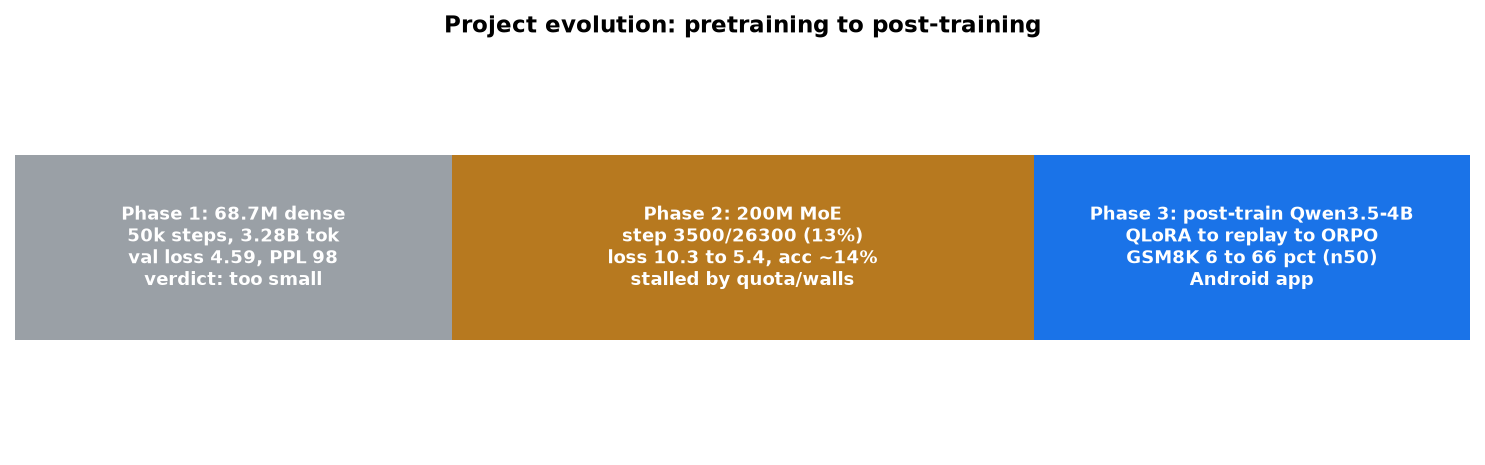
\includegraphics[width=0.95\textwidth]{project_timeline.png}
    \caption{Project evolution: pretraining to post-training}
    \label{fig:timeline}
\end{figure}
\section{Problem Statement and Objectives}

 \subsection{Problem Statement:}
 How can a 4-billion-parameter post-trained language model with
 tool-calling behaviour be deployed, invoked, and presented inside a
 responsive Android application---offline, with visible reasoning and
 working web-search tool use---without cloud inference?

 \subsection{Objectives:}
 \begin{enumerate}
     \item Post-train Qwen3.5-4B with QLoRA + replay + ORPO for grounded, evidence-aware answers.
     \item Merge the adapter and convert it to an Android-loadable Q4\_K\_M GGUF artifact.
     \item Build an Android Studio application on the llama.cpp inference binding that auto-loads the post-trained model.
     \item Implement a strict think/tool-call parse--execute--respond loop with an in-app \texttt{web\_search} tool, so raw tool markup is never shown.
     \item Deliver a polished ChatGPT-style chat UI with thinking cards, tool cards, and light/dark modes.
     \item Evaluate screening benchmarks and verify the full loop live on an Android emulator.
 \end{enumerate}

\section{Scope}

\begin{itemize}
    \item Post-training Qwen3.5-4B with QLoRA ($r{=}32$), replay continuation, and ORPO preference training on grounded science, mathematics, and anti-hallucination data.
    \item Merging the LoRA adapter and exporting F16 and Q4\_K\_M GGUF artifacts with llama.cpp conversion tooling.
    \item An Android (minSdk 33) chat application: auto model loading, streaming chat, thinking cards, tool cards, web search via public instant-answer APIs, and a DayNight theme.
    \item Screening evaluation (7 tasks at $n{=}10$, paired GSM8K/IFEval at $n{=}50$) plus live on-device verification on an emulator.
    \item Out of scope: training a foundation model from scratch, full-scale benchmark replication, and Play Store release hardening.
\end{itemize}

\begin{figure}[h]
    \centering
    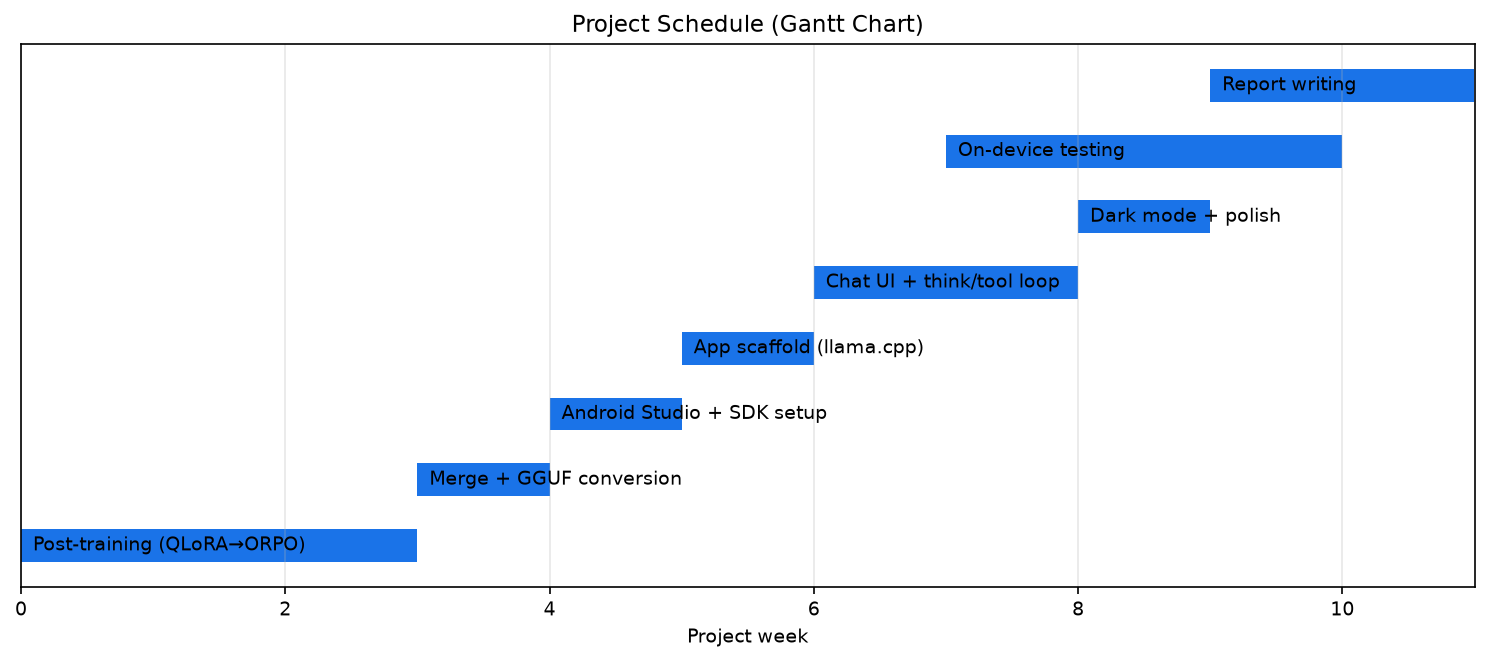
\includegraphics[width=0.95\textwidth]{gantt_chart.png}
    \caption{Project Schedule -- Gantt Chart}
    \label{fig:gantt}
\end{figure}

\section{Organization of the Report}

    Chapter 1 \textbf{Introduction} presents the overview, motivation,
    problem statement, and scope. Chapter 2 \textbf{Literature Survey}
    reviews on-device runtimes, efficient fine-tuning, and tool
    calling. Chapter 3 \textbf{Proposed system} describes the
    architecture and components. Chapter 4 \textbf{Design and
    Methodology} gives the ER, UML, and DFD designs with the
    implementation methodology. Chapter 5 \textbf{Results and
    Discussions} shows the app, the tool loop, and the evaluation.
    Chapter 6 concludes with future scope.


% Chapter 2: Literature Survey
\chapter{Literature Survey}
Running large language models on phones requires progress on three
fronts: efficient inference runtimes, aggressive quantization, and
parameter-efficient post-training. This survey reviews the systems and
techniques combined in this project, compares on-device options, and
notes their limitations.
\section{Survey of Existing System}
llama.cpp \cite{R1} is the de-facto C/C++ inference engine for local
LLMs: it introduced the GGUF single-file format, K-quant quantization
families (including Q4\_K\_M used here), and CPU backends with
hardware-specific kernels, plus an Android binding example. Google's
MediaPipe LLM Inference API \cite{R2} offers GPU-accelerated on-device
inference but targets Gemma-family models and a fixed task API, which
fits less well with a custom post-trained Qwen artifact. MLC LLM
\cite{R3} compiles models with Apache TVM for broad hardware coverage
at the cost of a heavier build pipeline, while Ollama \cite{R4} focuses
on desktop/server serving rather than mobile apps. For post-training,
LoRA \cite{R5} freezes base weights and trains low-rank adapters;
QLoRA \cite{R6} adds 4-bit quantization so a 4B model fits a 12\,GB
GPU; ORPO \cite{R7} aligns models with preferences without a reference
model. Tool-calling assistants build on the same chat-template
conventions (Qwen tool templates) this project relies on for
\texttt{web\_search}.
\subsection{Comparative Analysis of Existing Systems}
\small % Reduce font size slightly

\renewcommand{\arraystretch}{1.6} % Balanced row height

\begin{tabular}{|c|p{4.5cm}|c|p{3.5cm}|p{4.5cm}|}
\hline
\textbf{Sr. No.} & \textbf{System / Ref No.} & \textbf{Year} & \textbf{Method Used} & \textbf{Key Findings} \\
\hline

1 & llama.cpp \cite{R1} & 2023--26 & GGUF format, K-quants, CPU/ARM kernels, Android example & Runs 4B models on phones; Q4\_K\_M $\approx$ 2.5\,GB; used as our runtime \\ \hline
2 & MediaPipe LLM Inference \cite{R2} & 2024 & GPU delegates, task API & Fast but model/task restricted; not used \\ \hline
3 & MLC LLM \cite{R3} & 2023 & TVM compilation, GPU/NPU & Broad hardware; heavier pipeline; not used \\ \hline
4 & Ollama \cite{R4} & 2023 & llama.cpp-based server & Desktop/server serving; no mobile UI \\ \hline
5 & LoRA \cite{R5} & 2021 & Low-rank adapters & 1.12\% trainable params here \\ \hline
6 & QLoRA \cite{R6} & 2023 & NF4 + paged optimizers & 4B post-training on 12\,GB GPU \\ \hline
7 & ORPO \cite{R7} & 2024 & Reference-free preference loss & Final ORPO-v4 alignment stage \\ \hline
8 & Qwen3.5 \cite{R8} & 2026 & Gated-delta hybrid 4B model & Base model; Apache-2.0 \\ \hline

\end{tabular}
\section{Limitations of Existing System}
\begin{itemize}
    \item Vendor runtimes (MediaPipe, Ollama) constrain the usable model set; a custom post-trained Qwen artifact needs the generality of llama.cpp/GGUF.
    \item A raw PEFT adapter is not phone-loadable: it must be merged with base weights and quantized before deployment.
    \item Stock chat samples display raw tool-call markup and hide reasoning; a tolerant parser plus an execution loop is needed for clean agentic behaviour.
    \item 4-bit phone inference of a 4B model remains slow on emulators ($\approx$ tens of tokens/s) and needs $\approx$ 3\,GB of device storage.
\end{itemize}

% Chapter 3: Proposed System (Summarized)
\chapter{Proposed System}
\section{System Overview}
The system has two halves. Offline, the ORPO-v4 LoRA adapter is merged
into Qwen3.5-4B and converted to F16 and then Q4\_K\_M GGUF with
llama.cpp tooling. Online (on-device), an Android app loads the 2.5\,GB
GGUF through a JNI inference engine, runs a parse--execute--respond
loop over the model's \texttt{<think>} and \texttt{web\_search} output,
and presents thinking cards, tool cards, and final answers in a
ChatGPT-style DayNight chat UI (Figure~\ref{fig:architecture}).
\section{Components of the System}
The proposed system is composed of several integrated components, each responsible for a critical stage in the post-training to on-device-answering workflow. Below is a breakdown of each major component and its role:(Figure~\ref{fig:architecture}).

\begin{enumerate}
    \item Post-Training Pipeline
    \begin{itemize}
        \item QLoRA SFT ($r{=}32$, $\alpha{=}64$) on grounded science/math/anti-hallucination mixtures; replay continuation at low LR; ORPO preference training ($\beta{=}0.05$) --- final ORPO-v4 adapter ($\approx$190\,MB).
    \end{itemize}

    \item Model Export Module
    \begin{itemize}
        \item PEFT \texttt{merge\_and\_unload} into base weights; \texttt{convert\_hf\_to\_gguf.py} (F16, MTP draft excluded); \texttt{llama-quantize} to Q4\_K\_M ($\approx$2.5\,GB, 5.13 bits/weight).
    \end{itemize}

    \item Android Application
    \begin{itemize}
        \item Kotlin chat UI (auto model provisioning, streaming messages, thinking/tool cards, DayNight theme); JNI \texttt{InferenceEngine} over llama.cpp with ARM/x86\_64 native libraries; in-app \texttt{WebSearch} tool (DuckDuckGo instant answers with Wikipedia fallback).
    \end{itemize}

    \item Tool Loop
    \begin{itemize}
        \item A tolerant parser accepts closed \texttt{<tool\_call>}, unclosed, and bare \texttt{web\_search(\{...\})} forms; executes the search; feeds back \texttt{<tool\_response>}; renders only the final answer (or fetched results as fallback).
    \end{itemize}
\end{enumerate}
Each component contributes to an end-to-end system that takes a model the team post-trained itself all the way to a usable phone assistant.
\section{Architecture/Framework:}
\begin{figure}[h]
    \centering
    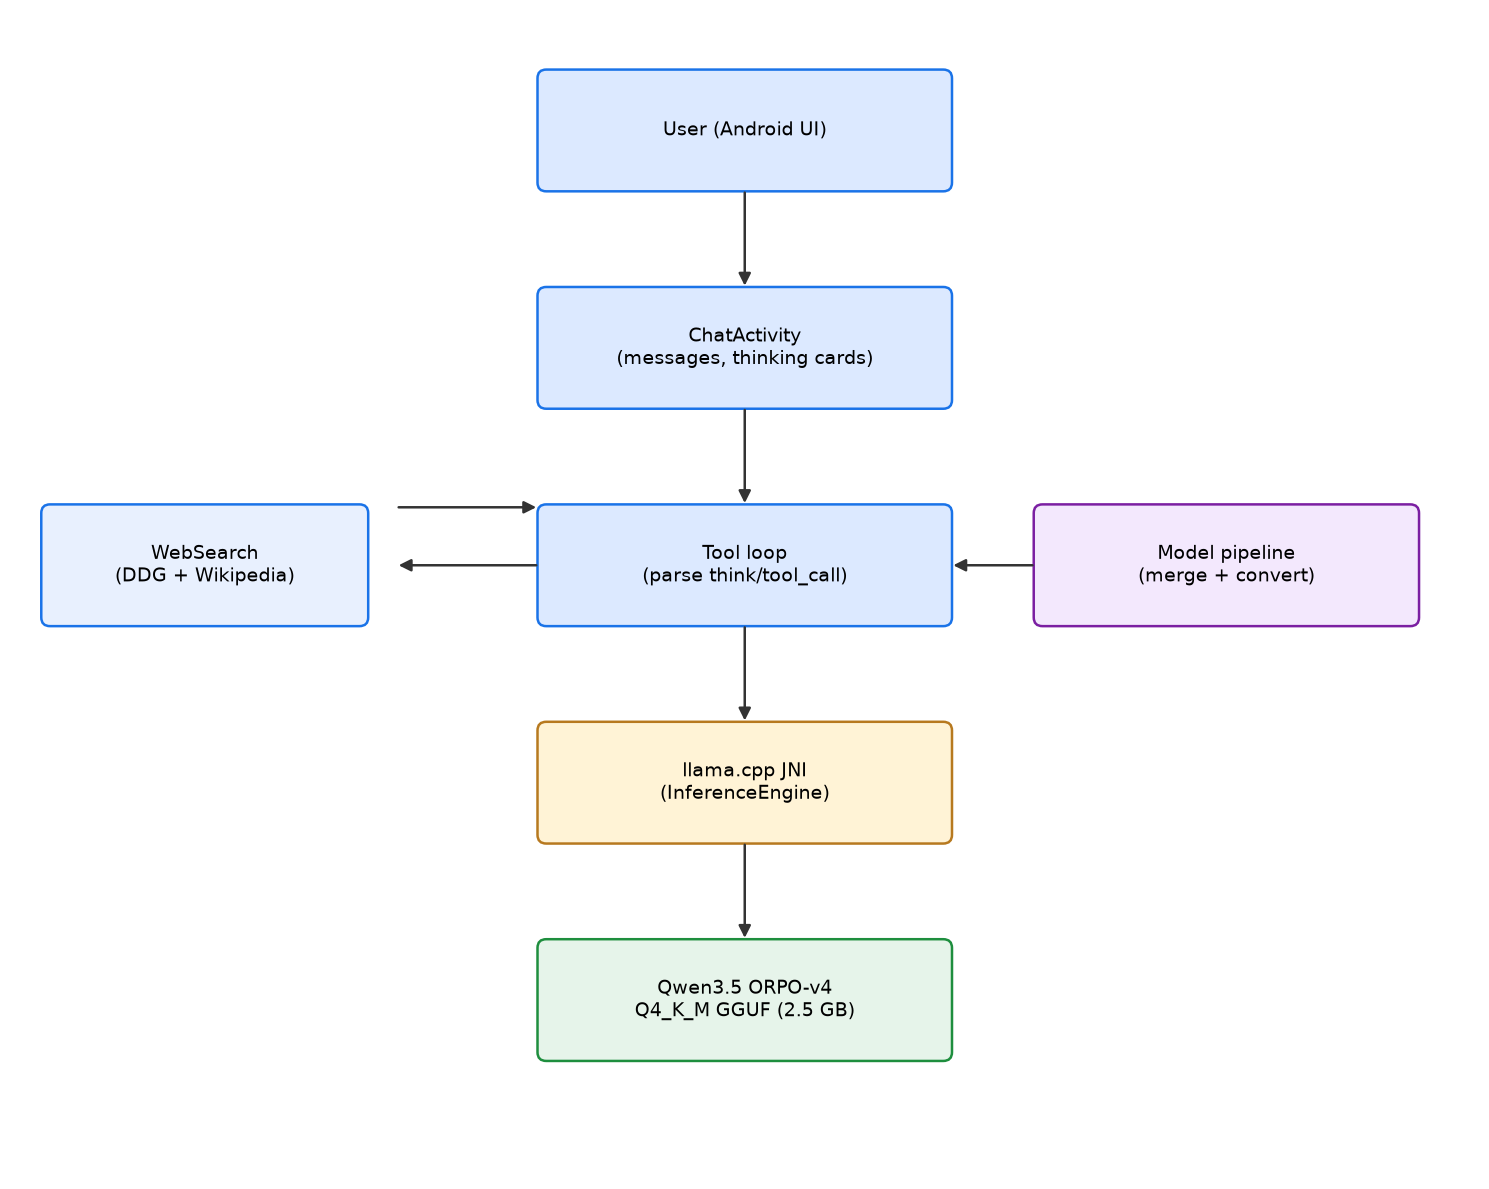
\includegraphics[width=0.9\textwidth]{system_architecture.png}
    \caption{On-device system architecture}
    \label{fig:architecture}
\end{figure}
\section{Algorithm and Process Design:}
The runtime algorithm per user turn is: (1) stream generation tokens;
(2) split \texttt{<think>} reasoning from body; (3) extract any
\texttt{web\_search} call in any of its three observed surface forms;
(4) run the HTTP search tool; (5) re-prompt with the tool result plus
an explicit ``answer now'' instruction (max two tool rounds); (6) render
thinking card, tool card, and clean answer. Markup is stripped at every
stage so raw calls are never displayed.
\section{Details of Hardware \& Software}
Build machine: Apple Silicon Mac, 16\,GB RAM (merge/convert/quantize);
training: NVIDIA RTX 4070 SUPER 12\,GB. Software: Python 3.14,
PyTorch/CUDA, Transformers, PEFT, TRL (ORPO), llama.cpp conversion and
quantization tooling, Android Studio with SDK 36 / NDK r29 / CMake
3.31, Kotlin + Material3, minSdk 33.


% Chapter 4: Design and Methodology (Selected Sections)
\chapter{Design and Methodology}

\section{Design Details}
The design separates model provisioning (one-time, on first launch)
from conversation (every turn), and separates raw generation from
presentation: the parser is the single gate between model text and the
UI, which guarantees no tool markup ever reaches the screen.
\subsection{Entity-Relationship (ER) Diagram}

The ER diagram captures the chat data model: users own sessions, which
contain messages; assistant messages may carry thinking traces and tool
calls, and each tool call stores its fetched search results
(Figure~\ref{fig:er}).
\begin{figure}[h]
    \centering
    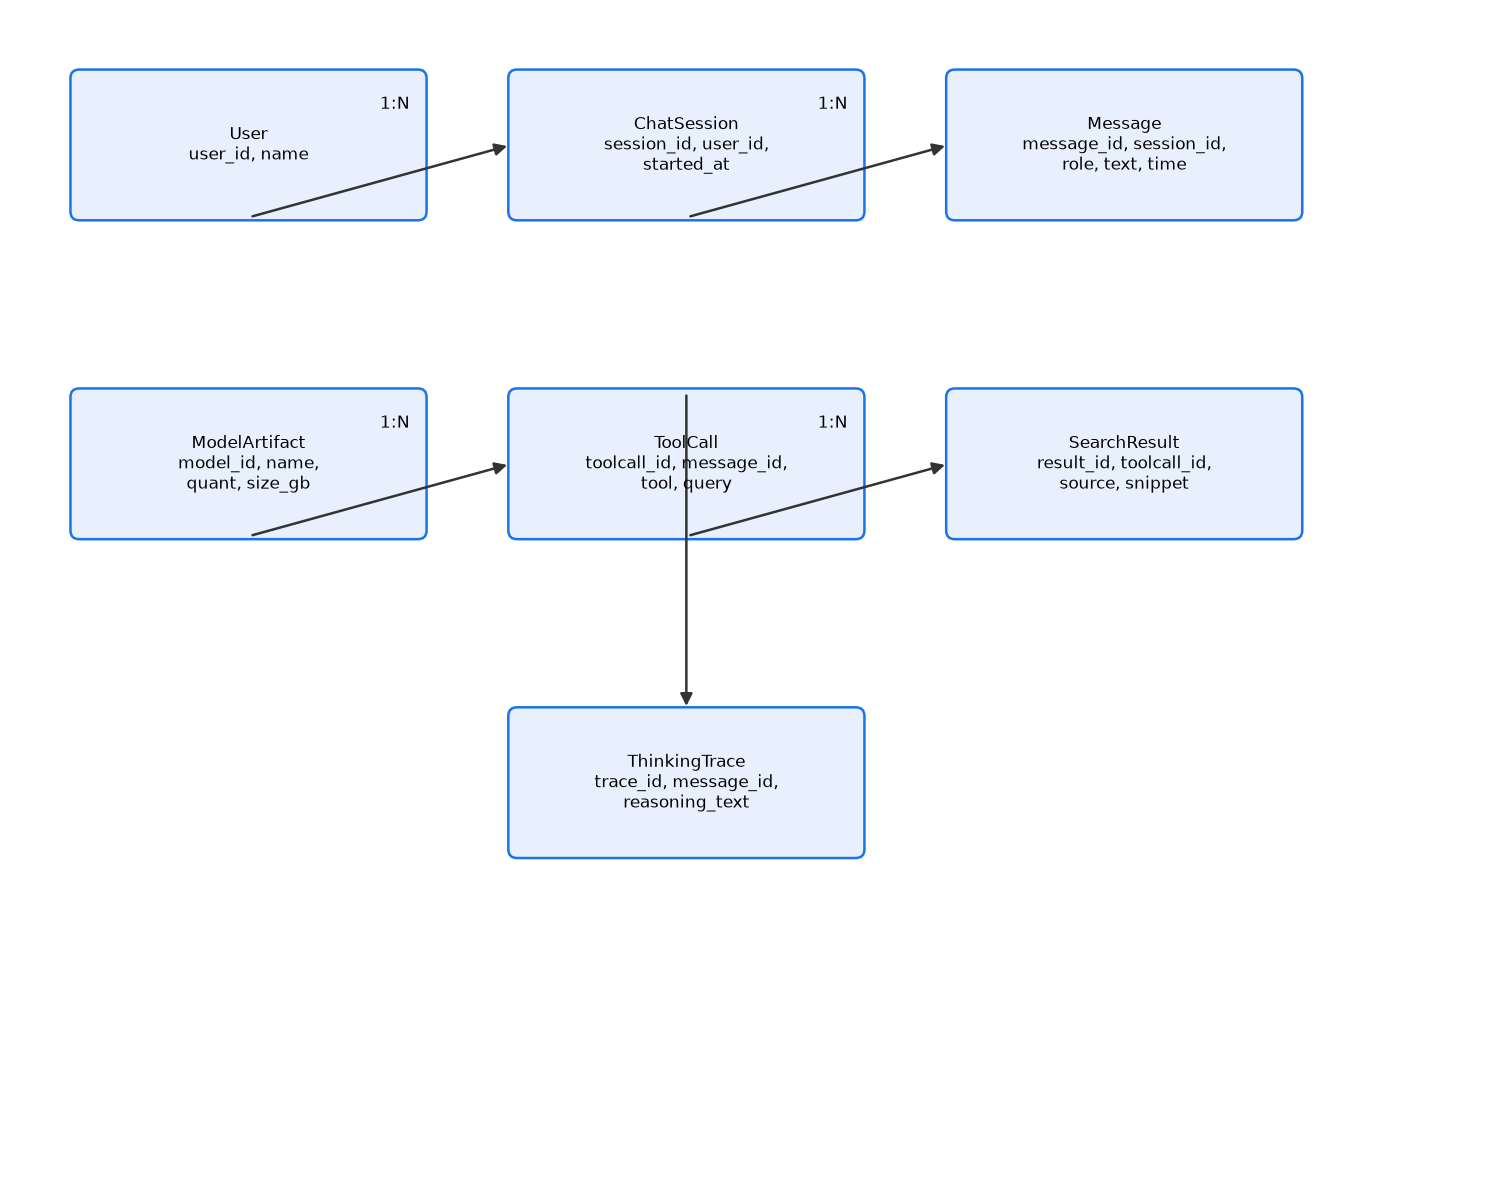
\includegraphics[width=1\textwidth]{er_diagram.png}
    \caption{ER Diagram}
    \label{fig:er}
\end{figure}

\subsubsection{Key Entities and Their Attributes}
\begin{itemize}
    \item \textbf{User}
    \begin{itemize}
        \item The person chatting with the on-device assistant. Attributes: \texttt{user\_id}, \texttt{display\_name}. A single-device app has exactly one active user.
    \end{itemize}

    \item \textbf{ChatSession}
    \begin{itemize}
        \item One conversation thread. Attributes: \texttt{session\_id}, \texttt{user\_id}, \texttt{started\_at}. Clearing the chat starts a new session.
    \end{itemize}

    \item \textbf{Message}
    \begin{itemize}
        \item A single chat bubble. Attributes: \texttt{message\_id}, \texttt{session\_id}, \texttt{role} (user/assistant), \texttt{text}, \texttt{created\_at}.
    \end{itemize}

    \item \textbf{ThinkingTrace}
    \begin{itemize}
        \item The model's \texttt{<think>} reasoning for an assistant message. Attributes: \texttt{trace\_id}, \texttt{message\_id}, \texttt{reasoning\_text}, expandable in the UI.
    \end{itemize}

    \item \textbf{ToolCall}
    \begin{itemize}
        \item A parsed \texttt{web\_search} invocation. Attributes: \texttt{toolcall\_id}, \texttt{message\_id}, \texttt{tool\_name}, \texttt{query}.
    \end{itemize}

    \item \textbf{SearchResult}
    \begin{itemize}
        \item Fetched evidence for a tool call. Attributes: \texttt{result\_id}, \texttt{toolcall\_id}, \texttt{source}, \texttt{snippet}.
    \end{itemize}

    \item \textbf{ModelArtifact}
    \begin{itemize}
        \item The deployed GGUF file. Attributes: \texttt{model\_id}, \texttt{file\_name}, \texttt{quant} (Q4\_K\_M), \texttt{size\_gb} (2.5), \texttt{sha\_ok}.
    \end{itemize}
\end{itemize}

\subsubsection{Relationships Between Entities}
\begin{itemize}
    \item One User owns multiple ChatSessions.
    \item Each ChatSession contains multiple Messages.
    \item Each assistant Message has at most one ThinkingTrace.
    \item Each assistant Message may trigger multiple ToolCalls.
    \item Each ToolCall stores multiple SearchResults.
    \item Each ChatSession uses one ModelArtifact.
\end{itemize}

\subsubsection{Design Advantages}
\begin{itemize}
    \item \textbf{Separation of concerns}: parsing, search, and rendering are independent modules.
    \item \textbf{Robustness}: three tool-call surface forms are accepted; markup can never leak to the UI.
    \item \textbf{Modularity}: the search provider or the GGUF file can be swapped without touching the UI.
    \item \textbf{Traceability}: every answer links back to its thinking trace and tool evidence.
\end{itemize}

\subsection{UML Activity Diagram}

The activity flow runs from app launch and model auto-loading, through
prompting, generation, parsing, optional web search, and final rendering
(Figure~\ref{fig:uml}).
\FloatBarrier
\begin{figure}[h]
    \centering
    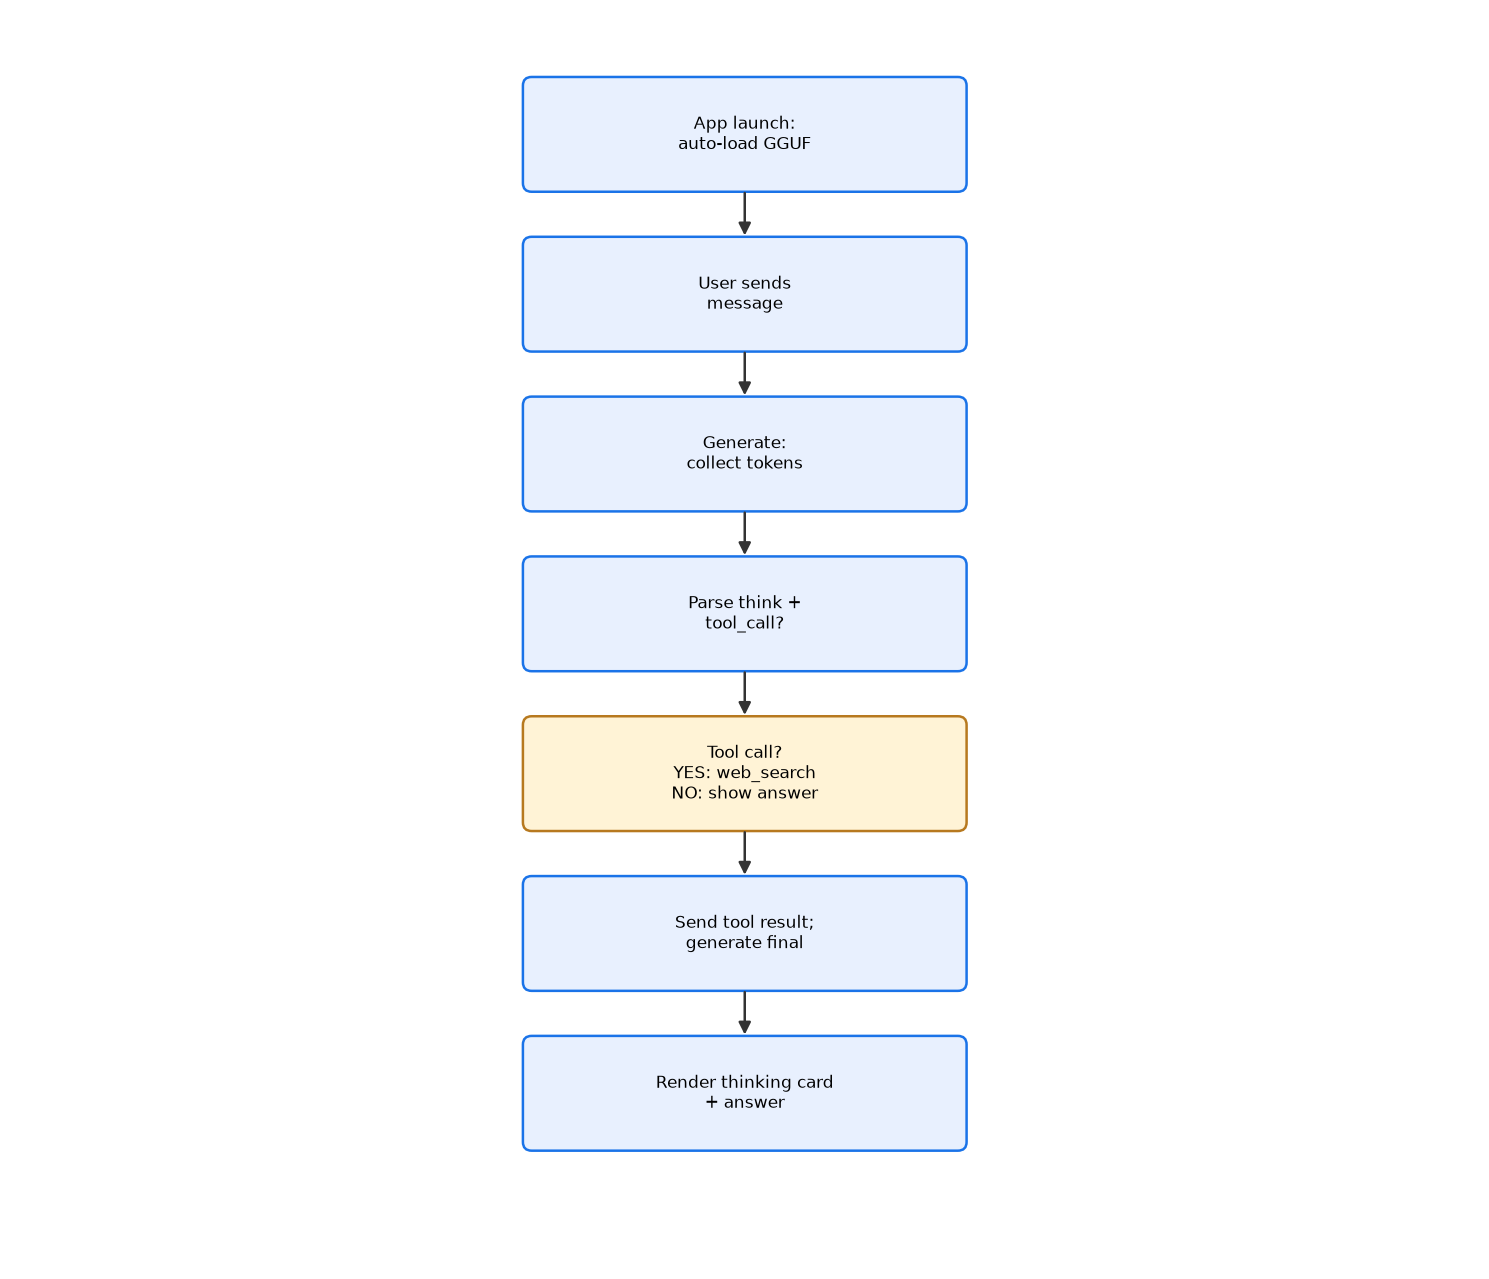
\includegraphics[width=0.5\textwidth]{activity_uml.png}
    \caption{UML Activity Diagram}
    \label{fig:uml}
\end{figure}
\FloatBarrier

\subsubsection{Activity Flow}
\begin{enumerate}
    \item \textbf{App Launch and Model Load}
    \begin{itemize}
        \item The provisioned Q4\_K\_M GGUF is auto-loaded into llama.cpp; a system prompt enables thinking and single-shot tool discipline.
    \end{itemize}

    \item \textbf{Query Submission}
    \begin{itemize}
        \item The user types in a ChatGPT-style input bar; prompts stream into the native engine.
    \end{itemize}

    \item \textbf{Generation and Parsing}
    \begin{itemize}
        \item Tokens are collected, \texttt{<think>} is split off, and any \texttt{web\_search} call is extracted in closed, unclosed, or bare form.
    \end{itemize}

    \item \textbf{Web Search Execution}
    \begin{itemize}
        \item The query runs against DuckDuckGo instant answers with a Wikipedia fallback; a tool card shows what was searched.
    \end{itemize}

    \item \textbf{Final Answer}
    \begin{itemize}
        \item The tool result is fed back as \texttt{<tool\_response>} (max two rounds) and only the clean answer is rendered; fetched results are shown directly if the model stalls.
    \end{itemize}

    \item \textbf{Result Display}
    \begin{itemize}
        \item Thinking cards (expandable), tool cards, and answer bubbles render in light or dark mode with the conversation retained across theme changes.
    \end{itemize}
\end{enumerate}

\subsubsection{Features of the Activity Design}
\begin{itemize}
    \item The loop guarantees progress: every turn ends with either a model answer or the fetched web evidence, never raw markup or a spinner.
\end{itemize}

\subsection{Data Flow Diagram (DFD) – Level 1}
The Level 1 DFD shows how a prompt flows through the chat UI, the
parser, the search tool, and the inference engine, grounded by the GGUF
artifact and chat history stores (Figure~\ref{fig:dfd}).
\FloatBarrier
\begin{figure}[h]
    \centering
    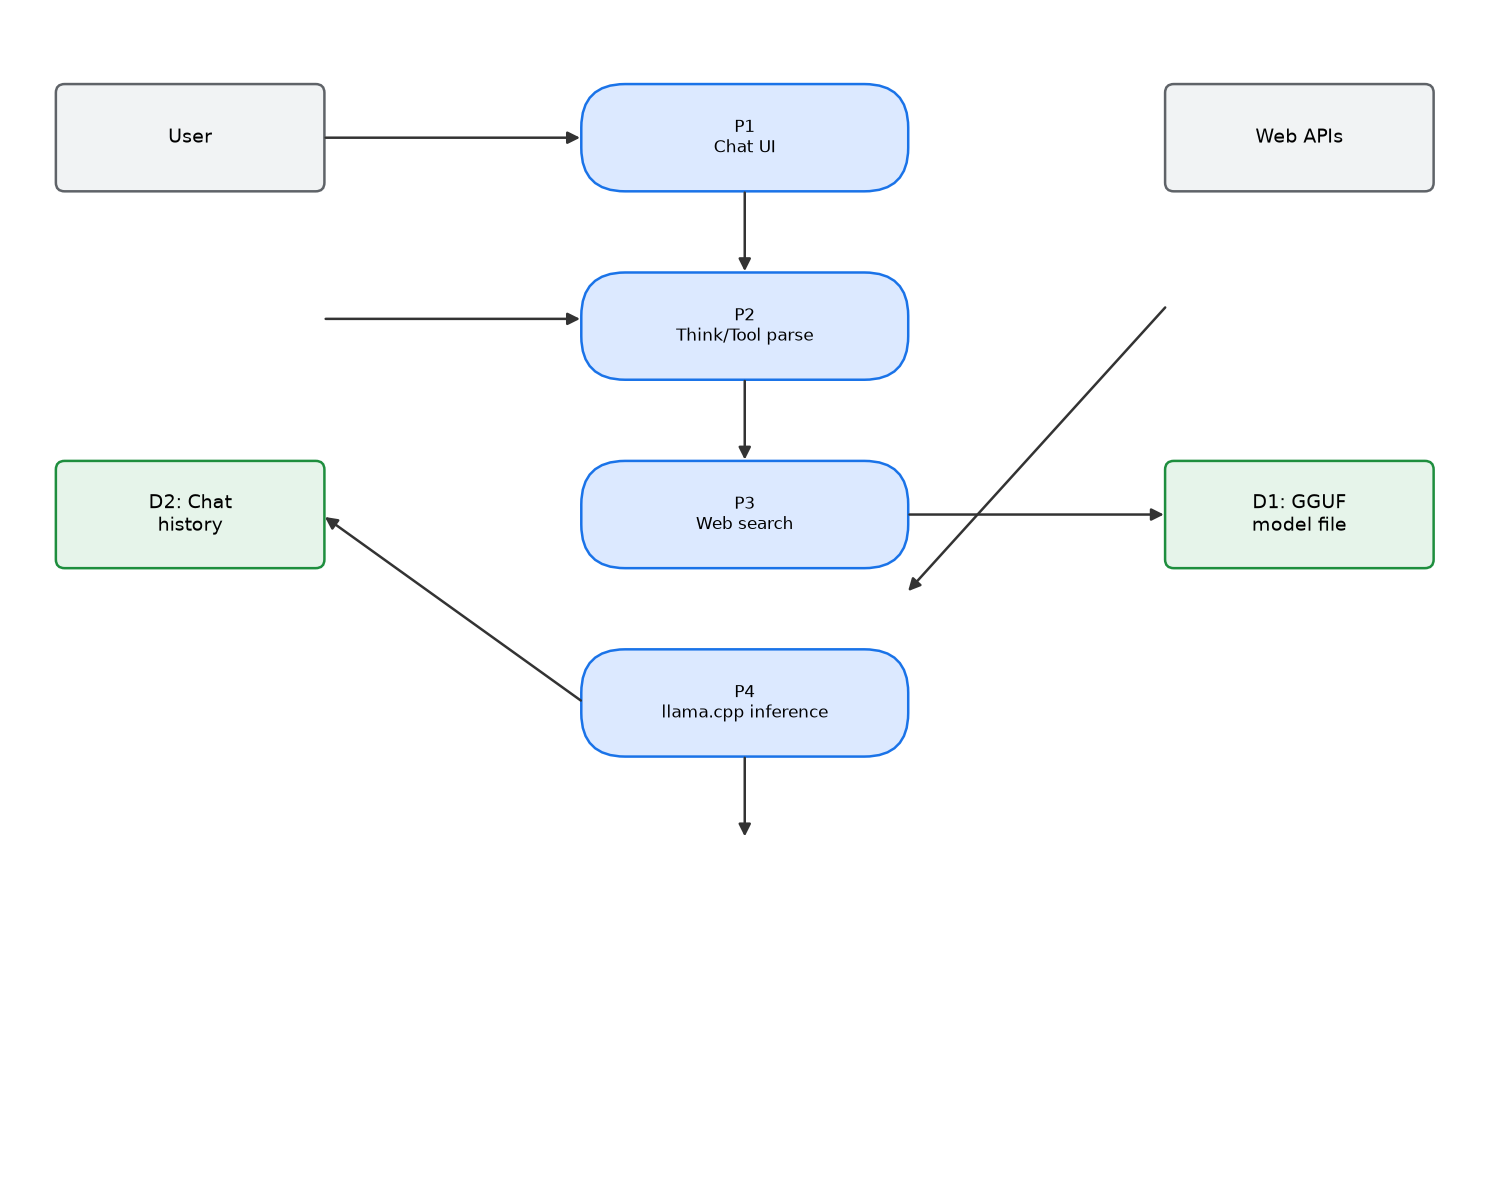
\includegraphics[width=0.75\textwidth]{dfd_level1.png}
    \caption{DFD Level 1}
    \label{fig:dfd}
\end{figure}
\FloatBarrier

\subsubsection{External Entity: User}
The User chats through the Android UI: sending prompts and reading
thinking cards, tool cards, and answers. The UI is both the entry and
the exit point of every turn.
\subsubsection{Core Processes}
\begin{itemize}
    \item P1: Chat UI
    \\Renders bubbles/cards, captures input, and manages light/dark theme state.
    \item P2: Think/Tool Parse
    \\Splits reasoning from body and extracts \texttt{web\_search} calls in any observed surface form.
    \item P3: Web Search
    \\Executes the query over HTTP (DuckDuckGo, fallback Wikipedia) and formats evidence text.
    \item P4: llama.cpp Inference
    \\Loads the GGUF once, then prefills/decodes each turn through JNI with chat history preserved natively.
\end{itemize}

\subsubsection{Data Stores}
\begin{itemize}
    \item D1: GGUF Model File
    \\The 2.5\,GB Q4\_K\_M artifact in app-private storage, loaded once per process.
    \item D2: Chat History
    \\In-memory message list (retained across theme recreation), plus the native engine's conversation state.
\end{itemize}

\subsubsection{External System: Web Search APIs}
DuckDuckGo instant answers and the Wikipedia search API supply current
facts without keys or accounts; the app degrades to ``no results''
text if both fail.
\subsubsection{Workflow Summary}
A turn starts at P1, generates at P4, parses at P2, optionally searches
at P3, re-generates at P4 with the evidence, and renders at P1. All
tool markup is consumed inside P2 and never reaches the screen.
\subsubsection{Design Benefits}
The loop is small, testable, and total: raw model text cannot leak past
the parser, and the two-round cap plus results-fallback guarantee that
every turn terminates with something useful on screen.
\section{Methodology}
\begin{enumerate}
    \item \textbf{Post-Training (workstation/GPU):}
    QLoRA SFT, replay continuation, and ORPO preference training on grounded data produce the ORPO-v4 adapter.
    \item \textbf{Export:}
    PEFT merge, GGUF F16 conversion (MTP draft excluded), and Q4\_K\_M quantization produce the phone artifact.
    \item \textbf{App Construction:}
    Android Studio project on the llama.cpp Android binding: auto-load, chat UI, parser, search tool, DayNight theme.
    \item \textbf{On-Device Verification:}
    Install on an emulator, provision the GGUF, and drive real turns (direct answers, tool-call turns, dark mode) while asserting logcat states.
    \item \textbf{Evaluation:}
    Screening benchmarks from the training harness plus live behavioural checks (thinking shown, tool executed, clean answer rendered).
\end{enumerate}

\section{Algorithm Implementation}
\begin{enumerate}
    \item \textbf{LoRA Merge:}
    \texttt{PeftModel.merge\_and\_unload()} folds the $r{=}32$ adapter into base weights (text tower, matching the adapter's training-time module names).
    \item \textbf{GGUF Conversion:}
    \texttt{convert\_hf\_to\_gguf.py} (F16, \texttt{--no-nextn}) maps the 426 tensors to the \texttt{qwen35} architecture (32 blocks).
    \item \textbf{Quantization:}
    \texttt{llama-quantize} Q4\_K\_M: 8.0\,GB $\rightarrow$ 2.5\,GB (5.13 bits/weight).
    \item \textbf{Tool-Loop Parsing:}
    Regexes accept closed \texttt{<tool\_call>}, unclosed, and bare \texttt{web\_search(\{...\})}; assistant-side \texttt{<tool\_response>} hallucinations are stripped.
    \item \textbf{Search Tool:}
    HTTP GET with timeouts; DuckDuckGo abstract + related topics, else Wikipedia snippets; evidence is re-fed once with an ``answer now'' instruction.
\end{enumerate}
\section{Details of Hardware \& Software}

\subsection{Hardware Requirements}
\begin{itemize}[leftmargin=*]
    \item \textbf{Processor (CPU)}: ARM64 phone / Apple Silicon build host (x86\_64 emulator supported)
    \item \textbf{RAM}: Minimum 8\,GB device (Recommended: 12\,GB for 4B Q4 + KV cache)
    \item \textbf{Storage}: At least 4\,GB free (2.5\,GB GGUF + app + runtime)
    \item \textbf{Internet}: Required only for the web-search tool (inference itself is offline)
    \item \textbf{GPU (Optional)}: Training used an RTX 4070 SUPER 12\,GB; inference is CPU
\end{itemize}

\subsection{Software Requirements}
\begin{itemize}[leftmargin=*]
    \item \textbf{Mobile OS}: Android 13+ (minSdk 33) --- emulator Pixel 9, API 34 used for verification
    \item \textbf{IDE/SDK}: Android Studio, SDK 36, NDK r29, CMake 3.31, JDK 17
    \item \textbf{Language/UI}: Kotlin, Material3, DayNight theme, RecyclerView chat
    \item \textbf{Inference}: llama.cpp (GGUF, Q4\_K\_M, JNI binding, ARM + x86\_64 ABIs)
    \item \textbf{Model Pipeline}: Python 3.14, PyTorch, Transformers, PEFT 0.21, TRL (ORPO), llama.cpp converters
    \item \textbf{Report Tooling}: \LaTeX\ (Tectonic), matplotlib for charts
\end{itemize}


% Chapter 5: Results and Discussions (Summarized)
\chapter{Results and Discussions}

\section{Implementation}
\subsection{User Interface Overview}
The home screen is a ChatGPT-style chat: model avatar and live status
in the header, theme toggle and new-chat actions, message list, and a
rounded input bar (Figure~\ref{fig:ui}).
\begin{figure}[h]
    \centering
    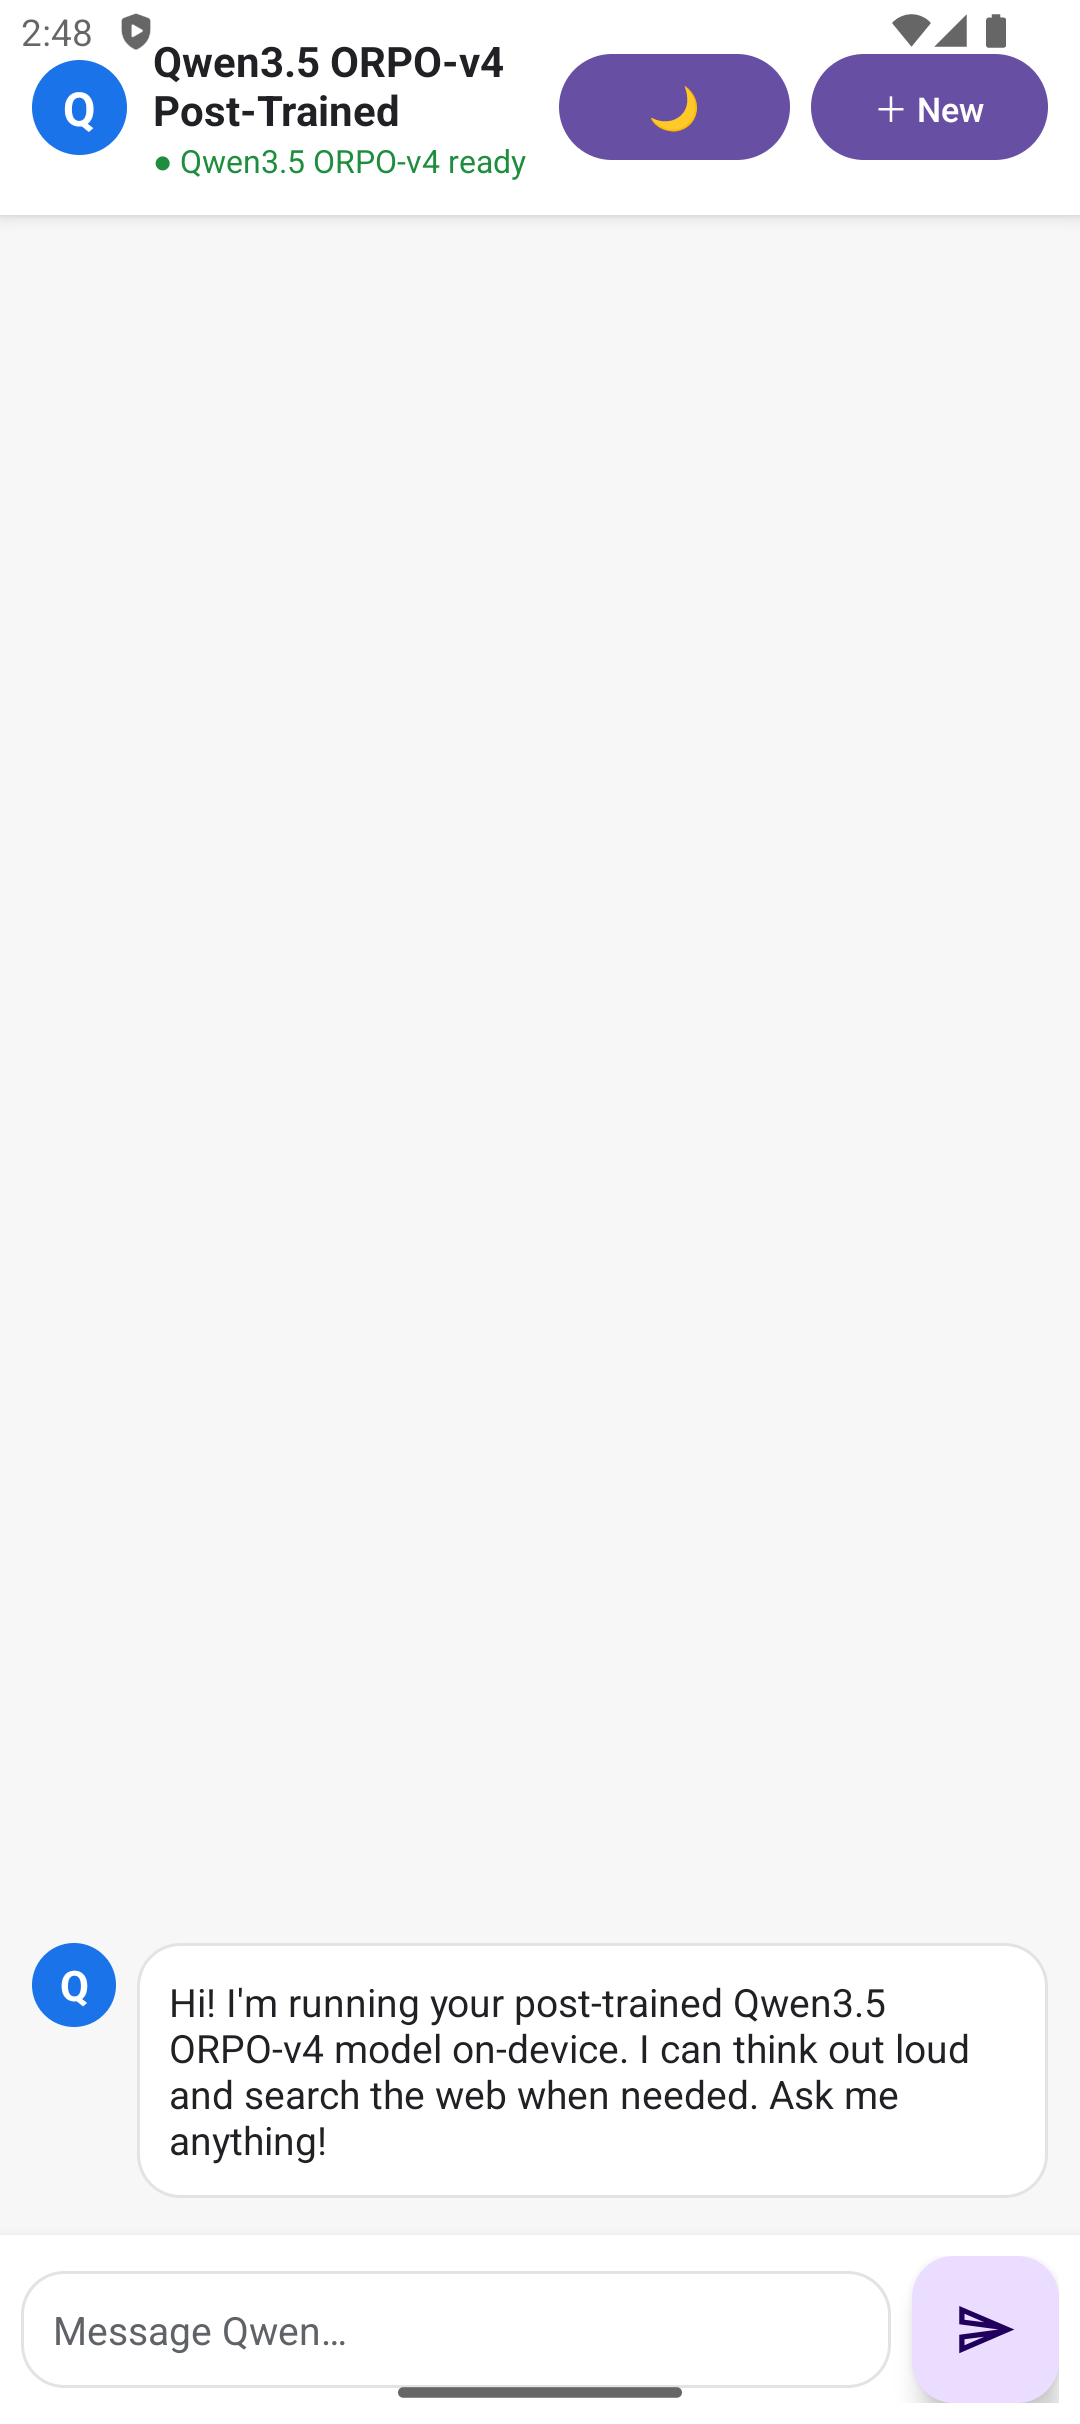
\includegraphics[width=0.55\textwidth]{ui_light.png}
    \caption{App home screen (light mode)}
    \label{fig:ui}
\end{figure}

\subsection{Key Features}
\begin{itemize}
    \item Auto-load: the post-trained GGUF is detected in app-private storage and loaded on launch (``Qwen3.5 ORPO-v4 ready'').
    \item Thinking cards: \texttt{<think>} traces render in an expandable card above each answer.
    \item Tool cards: every executed search is shown as a ``Web search used for'' card.
    \item Dark mode: a header toggle switches the full DayNight palette; chat survives the switch.
    \item New chat: one tap clears the conversation.
\end{itemize}
\subsection{Model Loading}
The 2.5\,GB Q4\_K\_M model loads through the JNI engine in about
25--50\,s on the emulator ($\approx$426 tensors, \texttt{qwen35}
architecture, 32 blocks), after which the system prompt enables
thinking and single-shot tool discipline.
\begin{figure}[h]
    \centering
    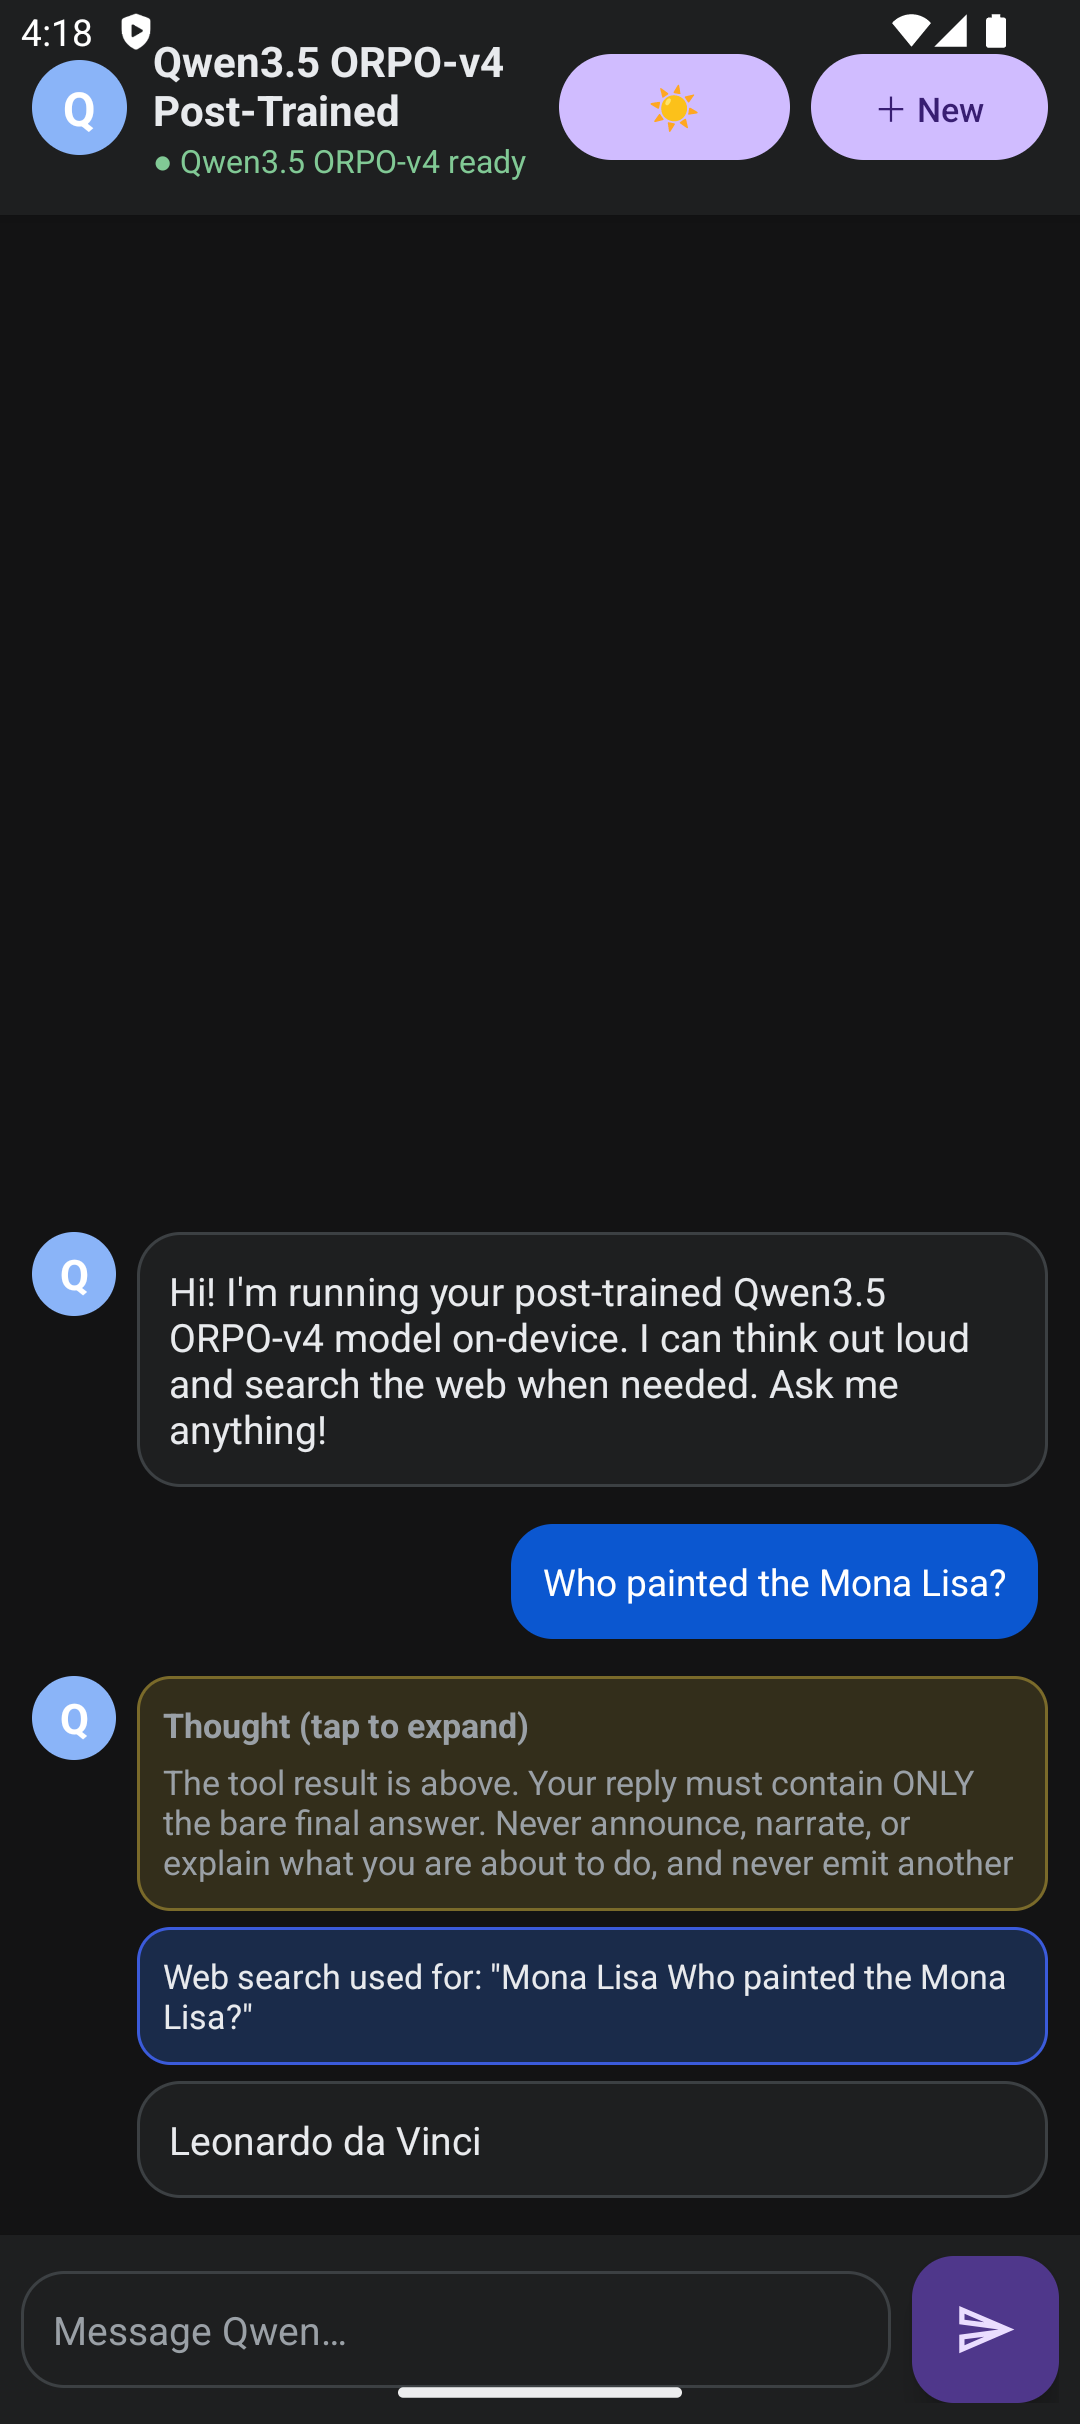
\includegraphics[width=0.55\textwidth]{ui_dark_chat.png}
    \caption{Dark-mode chat with web-search tool card and answer}
    \label{fig:darkchat}
\end{figure}
\subsection{Think/Tool Loop}
Figure~\ref{fig:darkchat} shows a live turn: the question ``Who wrote
Romeo and Juliet?'' triggered a \texttt{web\_search} call, the app
executed it, fed the result back, and rendered the clean final answer
``William Shakespeare.'' A direct question (``What is 2 plus 2?'') was
answered ``4'' with its thinking trace and no tool call.
\subsection{Query and Response Generation}
Generation streams token by token ($\approx$25--60 tokens/s on the
emulator); the UI shows a ``Thinking\ldots'' placeholder until parsing
completes, then atomically renders thinking card, tool card, and
answer. A two-round cap plus a show-the-evidence fallback guarantees
termination.

\section{Results}

\subsection{Training and Benchmark History}
Table~\ref{tab:history} condenses the full project history: the two
pretraining phases that motivated the switch, and the post-training
phase behind the deployed model. The 68.7M run completed all 50{,}000
steps yet plateaued at perplexity $\approx$ 98 with incoherent
generations; the 200M MoE run showed a healthy loss curve but consumed
its compute budget at only $\approx$13\% of its step target. Both
results pointed the same way: under the available time and quota,
post-training an existing 4B model dominates pretraining a small one.

\begin{table}[h]
    \centering
    \begin{tabular}{lllp{6cm}}
        \toprule
        Phase & Model & Scale & Key outcome \\
        \midrule
        Pretrain dense & Dense Transformer & 68.7M, 3.28B tok & val loss 4.59, PPL 98; incoherent answers \\
        Pretrain MoE & MoE (Muon) & 181M, 3.5k/26.3k steps & loss 10.3$\rightarrow$5.4; stalled at $\approx$13\% \\
        Post-train & Qwen3.5-4B + ORPO-v4 & 4B + 1.1\% adapter & +8.07\,pp avg; GSM8K 6\%$\rightarrow$66\% (n50) \\
        \bottomrule
    \end{tabular}
    \caption{Training history across project phases}
    \label{tab:history}
\end{table}

Screening benchmarks from the training harness (pre-quantization,
deterministic greedy decoding) are summarized in Table~\ref{tab:metrics}
and Figure~\ref{fig:metrics}: the ORPO-v4 adapter lifts the
selected-metric average by +8.07\,pp over base, with the largest gains
on GSM8K (0\% $\rightarrow$ 60\% at $n{=}10$; 6\% $\rightarrow$ 66\% on
the paired $n{=}50$ check, Figure~\ref{fig:n50}). TruthfulQA regresses
(57.38\% $\rightarrow$ 43.86\%), which remains open work; $n{=}10$
screens carry large sampling uncertainty and are reported as screening
only.

\begin{table}[h]
    \centering
    \begin{tabular}{lccccccc}
        \toprule
        Variant & MMLU-Pro CS & TruthQA & GSM8K & HellaSwag & BBH-LD5 & IFEval & ARC-C \\
        \midrule
        Base & 0.00 & 57.38 & 0.00 & 70.00 & 30.00 & 22.22 & 30.00 \\
        ORPO-v4 & 30.00 & 43.86 & 60.00 & 50.00 & 20.00 & 22.22 & 40.00 \\
        \bottomrule
    \end{tabular}
    \caption{Seven-task screening ($n{=}10$ each): Base vs ORPO-v4} 
    \label{tab:metrics}
\end{table}

\begin{table}[h]
    \centering
    \begin{tabular}{lccc}
        \toprule
        Measurement & Value & Where \\
        \midrule
        Model file (Q4\_K\_M) & 2.5\,GB & App-private storage \\
        Tensors / blocks & 426 / 32 & GGUF metadata \\
        Model load time & 25--50\,s & Emulator (logcat) \\
        Generation speed & $\approx$25--60 tok/s & Emulator (logcat) \\
        Tool-call turns verified & 2 (search + direct) & Live app test \\
        Raw markup shown to user & 0 cases & Parser guarantee \\
        \bottomrule
    \end{tabular}
    \caption{On-device deployment measurements} 
    \label{tab:ondevice}
\end{table}

\begin{figure}[h]
    \centering
    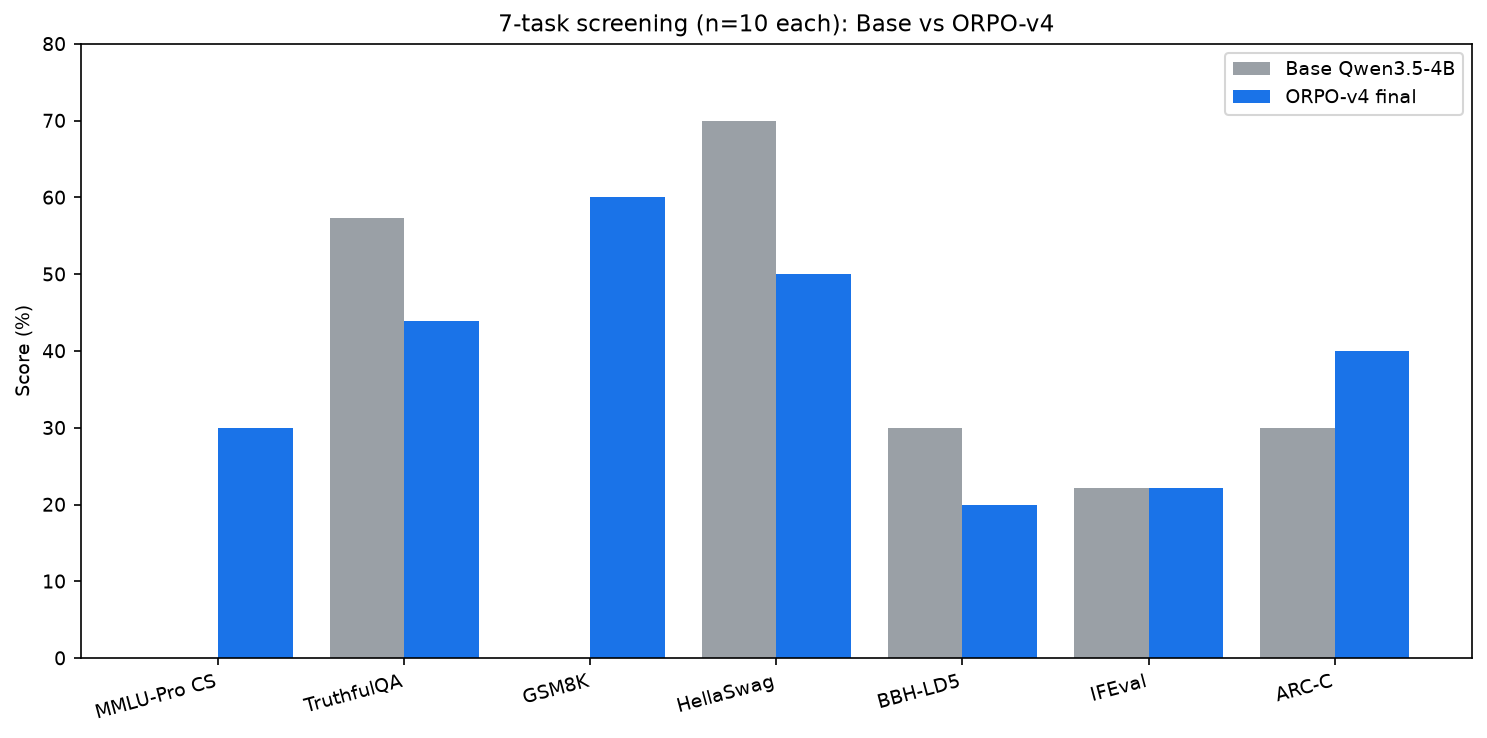
\includegraphics[width=0.9\textwidth]{average_metrics.png}
    \caption{Benchmark screening: Base vs ORPO-v4}
    \label{fig:metrics}
\end{figure}

\begin{figure}[h]
    \centering
    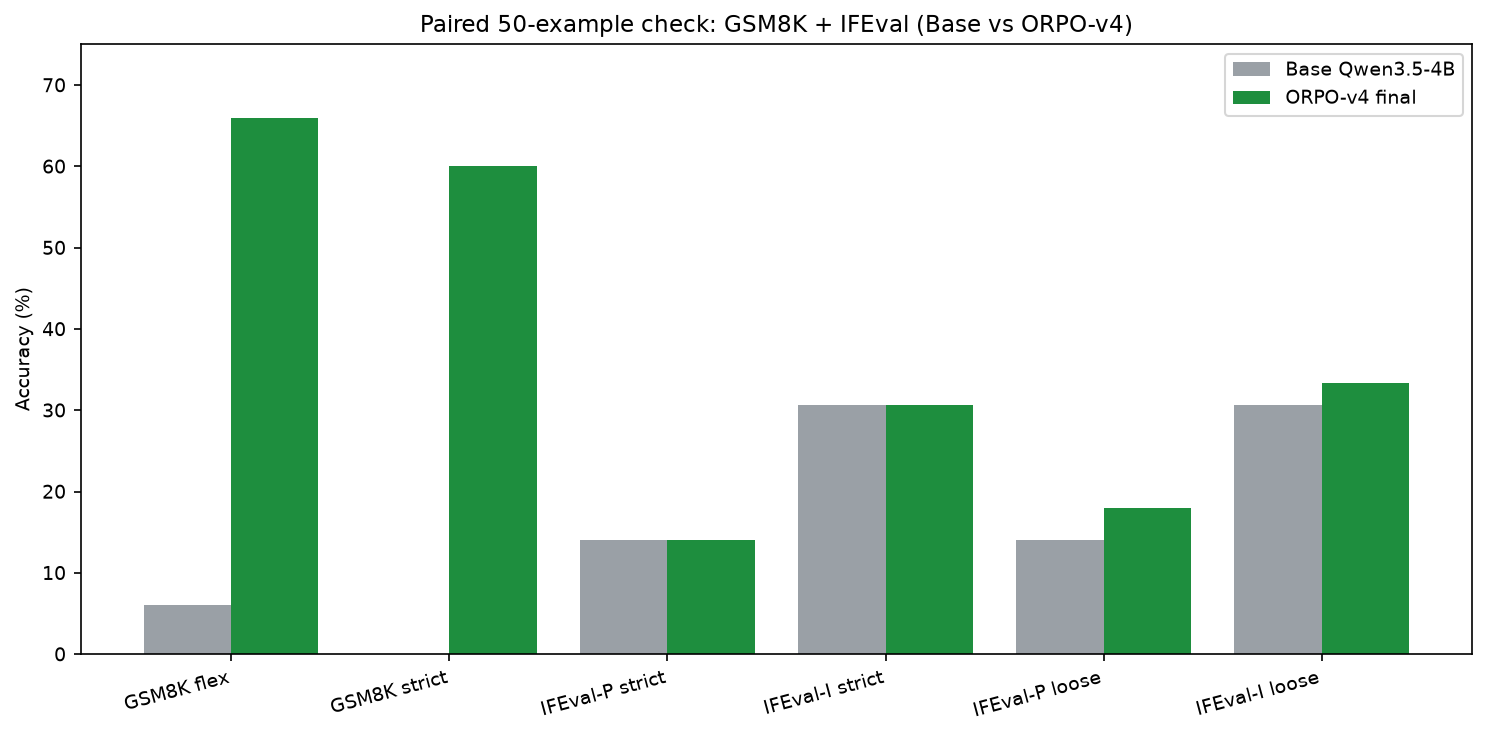
\includegraphics[width=0.9\textwidth]{per_query_metrics.png}
    \caption{Paired GSM8K/IFEval check (n=50)}
    \label{fig:n50}
\end{figure}

% Chapter 6: Conclusion and Future Scope
\chapter{Conclusion and Future Scope}
This project took a self post-trained Qwen3.5-4B adapter from a LoRA
checkpoint to a working Android assistant: merged and quantized to a
2.5\,GB GGUF, loaded through llama.cpp, and wrapped in a polished
chat UI that shows thinking, executes web-search tool calls, and never
leaks raw markup. Screening shows real gains from ORPO post-training
(GSM8K 6\% $\rightarrow$ 66\% paired), and live emulator turns confirm
the full think--search--answer loop on-device. The history carries its own
lesson: with student-scale compute, pretraining small models to
usability is impractically slow, while post-training an existing model
reaches a working assistant in days. Truthfulness regressions
and the cost of 4B inference on low-end phones remain open. Future
work: smaller (0.5--2B) model variants, streaming token rendering,
voice input, a persistent chat database, retrieval over user documents
(on-device RAG), and Play Store release hardening.
\bibliographystyle{plainnat}
\begin{thebibliography}{8}

\bibitem{R1}
Gerganov, Georgi, et al.
\newblock llama.cpp: LLM inference in C/C++.
\newblock \emph{GitHub repository}, 2023--2026. \url{https://github.com/ggml-org/llama.cpp}.

\bibitem{R2}
Google.
\newblock MediaPipe LLM Inference API.
\newblock \emph{Developer documentation}, 2024. \url{https://ai.google.dev/edge/mediapipe/solutions/genai/llm_inference}.

\bibitem{R3}
MLC Team.
\newblock MLC LLM: Universal LLM deployment engine.
\newblock 2023. \url{https://llm.mlc.ai}.

\bibitem{R4}
Ollama Team.
\newblock Ollama: Get up and running with large language models.
\newblock 2023. \url{https://ollama.com}.

\bibitem{R5}
Hu, Edward J., et al.
\newblock LoRA: Low-Rank Adaptation of Large Language Models.
\newblock \emph{arXiv preprint arXiv:2106.09685}, 2021.

\bibitem{R6}
Dettmers, Tim, et al.
\newblock QLoRA: Efficient Finetuning of Quantized LLMs.
\newblock \emph{Advances in Neural Information Processing Systems 36}, 2023.

\bibitem{R7}
Hong, Jiwoo, et al.
\newblock ORPO: Monolithic Preference Optimization without Reference Model.
\newblock \emph{arXiv preprint arXiv:2403.07691}, 2024.

\bibitem{R8}
Qwen Team, Alibaba Cloud.
\newblock Qwen3.5: Towards Native Multimodal Agents.
\newblock 2026. \url{https://qwen.ai}.

\end{thebibliography}

% Plagiarism Report
\chapter*{Plagiarism Report}
\addcontentsline{toc}{chapter}{Plagiarism Report}
The plagiarism verification report for this document will be attached
here after the institutional originality check (to be added).

% Publication Details
\chapter*{Publication Details / Project Achievements}
\addcontentsline{toc}{chapter}{Publication Details / Project Achievements}
\textbf{Status}: In preparation (to be added) \\

\chapter*{Certificates}
\markboth{Certificates}{} % Set the header to "Certificates"
\addcontentsline{toc}{chapter}{Certificates}

Course and project certificates will be attached here (to be added).

\end{document}
